\chapter{Arduino Startup}
\chaplabel{arduino}

\section{Installing the IDE}
We want to try installing the IDE at least two different ways. First, on the lab computer, then on your personal
computers if you have them. Both lab partners should try installing the software on the lab computer, each with 
their own login.

\subsection{Lab Computer}
This method may also work on your personal computers.
\begin{enumerate}
    \item On the search bar, type in Microsoft Store.
    \item Click on Microsoft Store
    \item In the store search, type arduino
    \item If you have the option to choose between version 1.x and 2.x, use 1.x.
    \item Arduino IDE App should appear, click on it
    \item Click on Get
    \item You do not need to sign into Microsoft to make this install work even if prompted
    \item Once it has installed, run the Arduino IDE app. 
	\item It should load up with a window that looks like Figure \ref{fig:emptysketch}.
	\item Try rebooting the computer, logging in and seeing if the Arduino app is still present.
\end{enumerate}

\begin{figure}[!htb]
	\centering
	\includegraphics[scale=1.0]{arduinoStart/emptysketch.PNG}
	\caption{This is what the Arduino IDE should load up to.}
	\label{fig:emptysketch}
\end{figure} 

\subsection{Personal Computer}
\begin{enumerate}
	\item Go to software download page: \href{https://www.arduino.cc/en/software}{https://www.arduino.cc/en/software}
	\item Scroll down to Legacy IDE (1.8.x)
	\item Download the Windows ZIP file (not the first link or the app) for 1.8.19
	\item Open the zip file and copy the folder inside (arduino-1.8.19 as of this writing) into your One Drive folder. This may take a while. If you are on your own computer, you can use any of the programs.
	\item Once that transfer finishes, go into the folder and run arduino.exe. Windows will try to save you, but if you click More Info you can click Run Anyway.
	\item Windows Defender Firewall will also complain. Uncheck the box that is checked and/or click Cancel.
	\item It should load up with a window that looks like Figure \ref{fig:emptysketch}.
\end{enumerate}

\section{Testing the Setup}
\subsection{Installing the Board Drivers}
\begin{enumerate}
	\item In order to get it to connect correctly to your board, you need to install the Arduino Nano Connect RP2040 board.
	\begin{enumerate}
		\item Navigate to Tools$\rightarrow$Board: ``Arduino Uno" (or similar)$\rightarrow$Boards Manager
		\item It should load as shown in Figure \ref{fig:boardsManager}.
        \begin{figure}[!htb]
            \centering
            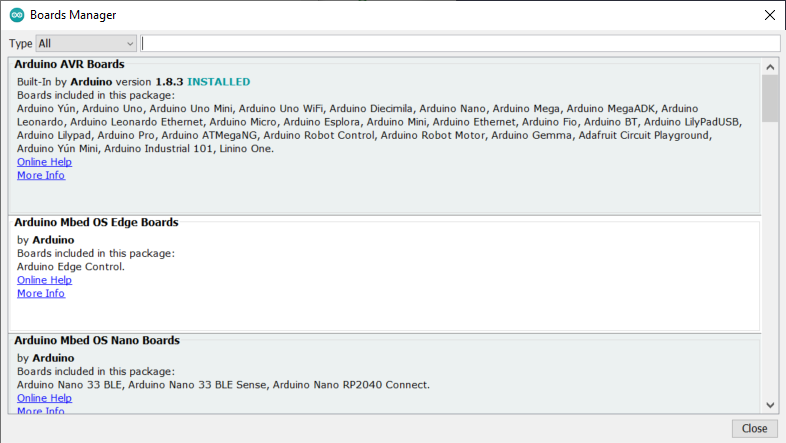
\includegraphics[scale=0.9]{arduinoStart/BoardsManager.PNG}
            \caption{This what the Boards Manager loads up to.}
            \label{fig:boardsManager}
        \end{figure} 
        \item In the search bar, type ``arduino nano connect" (without the quotes)
		\item The first item should be Arduino Mbed OS Nano Boards and should list the Arduino Nano RP2040 Connect.
		\item Move your cursor over it and it should show an Install button. Click it to install the board library.
		\item Wait for it to finish.
		\item While you are waiting, plug your Nano Connect into your computer and let it install it.
		\item As it finished, I received a User Account Control warning asking if I wanted to let dpinst-amd64.exe make changes to my device. I said yes.
		\item Next it asked me if I wanted to install Arduino Universal Serial Bus devices. Again, click to Install.
		\item It popped up again and I clicked Install again. Now it should say that the Arduino Mbed OS Nano Boards has been installed.
		\item Close the Boards Manager.
	\end{enumerate}
\end{enumerate}

\subsubsection{Compiling, Uploading, and Running}
This section can be done on either (or both) computers. The results from one run (between both lab partners)
is all that needs to be turned in.
\begin{enumerate}
	\item Now go to Files$\rightarrow$Examples$\rightarrow$01.Basics$\rightarrow$Blink.
	\item This will open another window with the Blink program.
	\item Go to Tools$\rightarrow$Board$\rightarrow$Arduino Mbed OS Nano Boards and select the Arduino Nano RP2040 Connect
	\item Go to Tools$\rightarrow$Port and select the COM that isn't COM1 (mine showed up as COM5)
	\item Click the right arrow under the word edit in the menu to Upload the sketch to the Arduino board.
	\item It should say ``Compiling sketch..." in the lower left and show a progress bar on the lower right.
	\item Then it should switch to Uploading... and finally Done Uploading.
	\item An orange light near the USB port on your board should be blinking.
	\item Congratulations! You have programmed your board!
	\item Now look in the program for the two delay statements. Try changing the values inside the parentheses and re-uploading it. Does the blinking change?
	\item In order to save files and have it portable, you need to change the directory where the Arduino IDE stores it's sketchbooks
	\begin{enumerate}
		\item Go to File$\rightarrow$Preferences
		\item Change the Sketchbook location to your OneDrive and a folder named arduino (lowercase is good)
		\item My OneDrive was in \\C:\textbackslash Users\textbackslash mcneils2\textbackslash OneDrive - Embry-Riddle 
		Aeronautical University\textbackslash arduino
	\end{enumerate}
	\item Now try saving the blink sketch with your changed values.
	\item Demonstrate your working blink and it's storage location to your instructor/TA
	\item Here are some other Examples to test:
	\begin{enumerate}
		\item Basics $\rightarrow$ fade: change the variable \lstinline|led| to have the value 
            \lstinline|LED_BUILTIN|, watch the red/orange LED pulse
%		\item Analog $\rightarrow$ AnalogInOutSerial: change analogInPin to A1 and analogOutPin to LED\_BUILTIN. Turn 
%				the potentiometer (R6) with a screwdriver and watch the LED change accordingly. If you press the magnifying
%				glass button in the top right the actual values will scroll by. You may need to set the baud rate to 9600.
		\item Digital $\rightarrow$ DigitalInputPullup: Change the first pinMode call to use A0 instead of 2. The same for 
				the digitalRead command (2$\rightarrow$A0). Press the right button (SW1) and see the LED blink. 
				 Note that this program isn't written as well as the others since you have to change a number in two
				places. Could you rewrite it better?
	\end{enumerate}
    \item Finally, create a sketch called \lstinline$getIDs$ using the code at \\ 
        \href{https://github.com/semcneil/CEC325Examples/blob/main/getIDs/getIDs.ino}{https://github.com/semcneil/CEC325Examples/blob/main/getIDs/getIDs.ino}
    \item You will need to install two libraries to make this script run.
    \begin{enumerate}
        \item Go to Sketch $\rightarrow$ Include Library $\rightarrow$ Manage Libraries 
        \item Install the ArduinoECCX08 and OneWireNG (only version 0.12.2 or earlier) libraries
    \end{enumerate}
    \item Run \lstinline$getIDs$ and submit the results in the end of lab Canvas quiz. The results will be 
                in the Serial Monitor which can be accessed through Tools$\rightarrow$Serial Monitor or the 
                button in the top right of the IDE. Don't forget that \lstinline$getIDs$ requires two libraries:
        \begin{enumerate}
            \item ArduinoECCX08
            \item OneWireNg version 0.12.x. Version 0.13.x doesn't work
        \end{enumerate}
\end{enumerate}


\section{Turn In}
\begin{enumerate}
    \item Make sure that the TA or instructor has signed off on your modified blink sketch.
    \item Submit a PDF of your edited blink.ino and the .ino of your blink sketch. The easiest way
            to create a PDF is to print to PDF. Only one 
            submission per group is required but make sure that both your names are on the sketch.
    \item Fill out the end of lab quiz prior to leaving. Note that it includes asking you 
            for the output of the \lstinline$getIDs$ sketch. Both group members should complete
            this quiz.
\end{enumerate}
